\section{Usuario}
\subsection{Representación}

\begin{frame}{Usuario}
	\begin{block}{Representación}
		Un usuario quedará identificado por su idUser, los usuarios se guardarán en una carpeta especial con
		ficheros como el siguiente.
	\end{block}
	
	\begin{exampleblock}{0.usr}
	\begin{columns}
		\column	{.35\textwidth}
		\lstinputlisting{../.chatConfig/users/0.usr}
		
		\column	{.65\textwidth}
		\begin{itemize}
			\item Identificador de usuario
			\item Nombre de usuario
			\item Contraseña
			\item Grupos a los que pertenece
		\end{itemize}	
	\end{columns}
	\end{exampleblock}
\end{frame}


% -----------------------------------

\subsection{Conversaciones}
\begin{frame}{Conversaciones}
	\begin{block}{Mensajes}
	Los mensajes tienen un identificador del grupo al que pertenecen, del usuario que los envía y un identificador del mensaje. Estos tres parámetros formarán la clave primaria, también se incluirá la fecha del envío del mensaje y el nombre del usuario que lo envía.
	\end{block}
	
	\begin{exampleblock}{ }
		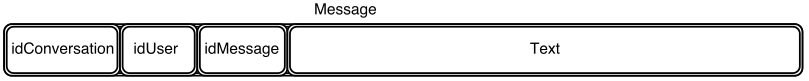
\includegraphics[scale=0.43]{./Imagenes/message.png}
	\end{exampleblock}
\end{frame}


% -----------------------------------


\begin{frame}{Fichero conversación}
	\begin{block}{ }
		Un fichero de conversación será una sucesión de mensajes.
	\end{block}
	
	\begin{exampleblock}{example.chat}
		\begin{figure}[H]
		\lstinputlisting{../.chatConfig/conversations/example.chat}
		\end{figure}
	\end{exampleblock}
\end{frame}


% -----------------------------------

\subsection{Mejoras posibles}
\subsection{Varias personas en un chat}
\begin{frame}{Mejoras}
	\begin{block}{Varios chats del mismo usuario}
		Para tener varios chats podríamos usar:
		
		\begin{itemize}
			\item Varios Printer por usuario
			\item Un único Printer que guarda las conversaciones en archivos
		\end{itemize}
	\end{block}
	
	\begin{block}{Grupos}   
		En este caso el cliente actuaría también como servidor que recibe los mensajes del servidor principal y los muestra por pantalla.
	\end{block}
\end{frame}


% -----------------------------------